\documentclass{revtex4}
\usepackage{hyperref}
\usepackage{graphicx}
\begin{document}

\title[scater supplementary figures]{Supplementary Figures---``\emph{scater:} pre-processing, quality control, normalisation and visualisation of single-cell RNA-seq data in R''}
\author{Davis J.~McCarthy\,$^{\text{1,2,5}*}$, Kieran R.~Campbell\,$^{\text{2,4}}$, Aaron T.~L.~Lun\,$^{\text{6}}$ and Quin F.~Wills\,$^{\text{2,3}}$}
\address{$^{\text{1}}$European Molecular Biology Laboratory - European Bioinformatics Institute (EMBL-EBI), Hinxton CB10 1SD, United Kingdom;\\
$^{\text{2}}$Wellcome Trust Centre for Human Genetics, University of Oxford,
Roosevelt Drive, Oxford OX3 7BN, United Kingdom;\\
$^{\text{3}}$Weatherall Institute for Molecular Medicine, University of Oxford, John Radcliffe Hospital, Oxford OX3 9DS, United Kingdom;\\
$^{\text{4}}$Department of Physiology, Anatomy and Genetics, University of Oxford, South Parks Road, Oxford OX1 3QX, United Kingdom;\\
$^{\text{5}}$St Vincent's Institute of Medical Research, 41 Victoria Parade, Fitzroy Victoria 3065, Australia; and \\
$^{\text{6}}$CRUK Cambridge Institute, University of Cambridge, Robinson Way, Cambridge CB2 0RE, United Kingdom.
% $^{\text{\sf 4}}$Department of Statistics, University of Oxford, Oxford, Oxfordshire, UK;
}

\begin{abstract}
Supplementary material and figures---details of package dependencies; an overview of the SCESet class; an overview of the \emph{scater} ecosystem; examples of using the \emph{scater} GUI.\\ \\
\textbf{Contact:} \href{davis@ebi.ac.uk}{davis@ebi.ac.uk}
\end{abstract}


\maketitle


\section*{Details of package dependencies}

The package builds on many other R packages: \emph{Biobase} and \emph{BiocGenerics} for core Bioconductor functionality  \citep{Huber2015-en}; \emph{plyr} \citep{Wickham2015-kj}, \emph{reshape2} \citep{Wickham2012-ec}, \emph{dplyr} \citep{Wickham2015-la}, \emph{data.table} \citep{Dowle2015-zc} and \emph{magrittr} \citep{Bache2014-sa} for reading and
tidying data; \emph{ggplot2} \citep{Wickham2016-dc} for plotting; \emph{biomaRt} \citep{Durinck2005-yz} for feature annotation; \emph{edgeR} \citep{Robinson2010-ky} for computation of normalisation size factors and counts-per-million values; \emph{limma} \citep{Ritchie2015-so} for efficient fitting of linear models to features; \emph{rhdf5} \citep{Fischer2016-me}, \emph{rjson} \citep{Couture-Beil2014-kk} and \emph{tximport} \citep{Soneson2015-fw} for reading in transcript-level expression values;
\emph{viridis} \citep{Garnier2016-hk} for perceptually-uniform colour
maps for plotting; \emph{parallel} for parallel computation; \emph{matrixStats} \citep{Bengtsson2016-tn} for computation of summary statistics from matrices; \emph{cowplot} \citep{Wilke2016-hj} for attractive plotting themes; \emph{destiny} \citep{Angerer2015-sw} for producing diffusion maps; \emph{Rtsne} \citep{Krijthe2015-is} for producing t-SNE plots; \emph{mvoutlier}
\citep{Filzmoser2015-kx} for multivariate outlier detection from PCA of QC metrics; \emph{roxygen2} \citep{Wickham2015-pu}, \emph{BiocStyle} \citep{Huber2015-en}, \emph{knitr} \citep{Xie2013-bn} and \emph{rmarkdown} \citep{Allaire2016-dl} for generating documentation; and \emph{testthat} \citep{Wickham2011-cj} for unit testing. As well as functioning in the usual R environments, \emph{scater} also has a GUI built using
\emph{shiny} \citep{Chang2016-of} and \emph{shinydashboard} \citep{Chang2015-bn} for intuitive and interactive data visualisation. Calling the \verb|scater_gui| function from within an R session opens up the GUI in a web browser.


\section*{Entry points for third-party tools from \emph{scater}}

The \emph{scater} package serves to prepare data for a wide variety of downstream analyses with third-party tools. Given the diverse nature of analyses that can be done with scRNA-seq data, the entry points for various third-party tools in terms of data preparation and transformation/format can vary. Below we discuss entry points from \emph{scater} into example third-party tools representing major categories of downstream analysis.

\paragraph{Differential expression analysis with \emph{scde} or \emph{edgeR}} Differential expression analysis tools for RNA-seq data, including \emph{scde} and \emph{edgeR} take raw counts as input data and can handle known batch effects in their statistical models. Therefore, the upstream data processing with \emph{scater} is straightforward: QC on cells and genes should be carried out with \emph{scater} as usual, and the count data supplied to the DE tool. Accessing the count matrix is as simple as applying the counts() function to an SCESet object. For an \emph{edgeR} analysis, size-factors computed with \emph{scran} should also be supplied, and the convertTo function from \emph{scran} makes it very easy to convert an SCESet object from a \emph{scater} workflow to a DGEList object needed for an \emph{edgeR} analysis.

\paragraph{Clustering with \emph{SC3}} Clustering results can be negatively impacted by the inclusion of poor quality cells, so QC of cells and genes as usual with \emph{scater} is necessary before supplying data to a clustering algorithm. In general, clustering algorithms do not account internally for batch effects and similar, so it will often be desirable to normalise expression data with size factors and regress out known batch effects or other technical effects. In the case of clustering with \emph{SC3}, a QC'd and normalised SCESet object can be supplied directly to the sc3 function for clustering.

\paragraph{Pseudotime estimation with \emph{monocle}} As with clustering, current pseudotime estimation methods do not internally account for batch effects. Thus, before applying pseudotime tools, data should be QC'd with \emph{scater} to remove problematic cells and genes. Size-factor normalisation of data is advisable, and the normaliseExprs function in \emph{scater} can be used to regress out known batch or technical effects. Once a filtered and normalised SCESet object has been obtained, the convertTo function in \emph{scran} can be used to convert the SCESet object to a CellDataSet object used in \emph{monocle}.

The three examples above demonstrate that the QC steps in \emph{scater} are necessary before any downstream analyses. The entry point from \emph{scater} varies for different third-party tools, but is nevertheless straightforward in most cases.


\section*{Supplementary Figures}


\begin{figure}[!tpb]%figure2
\centerline{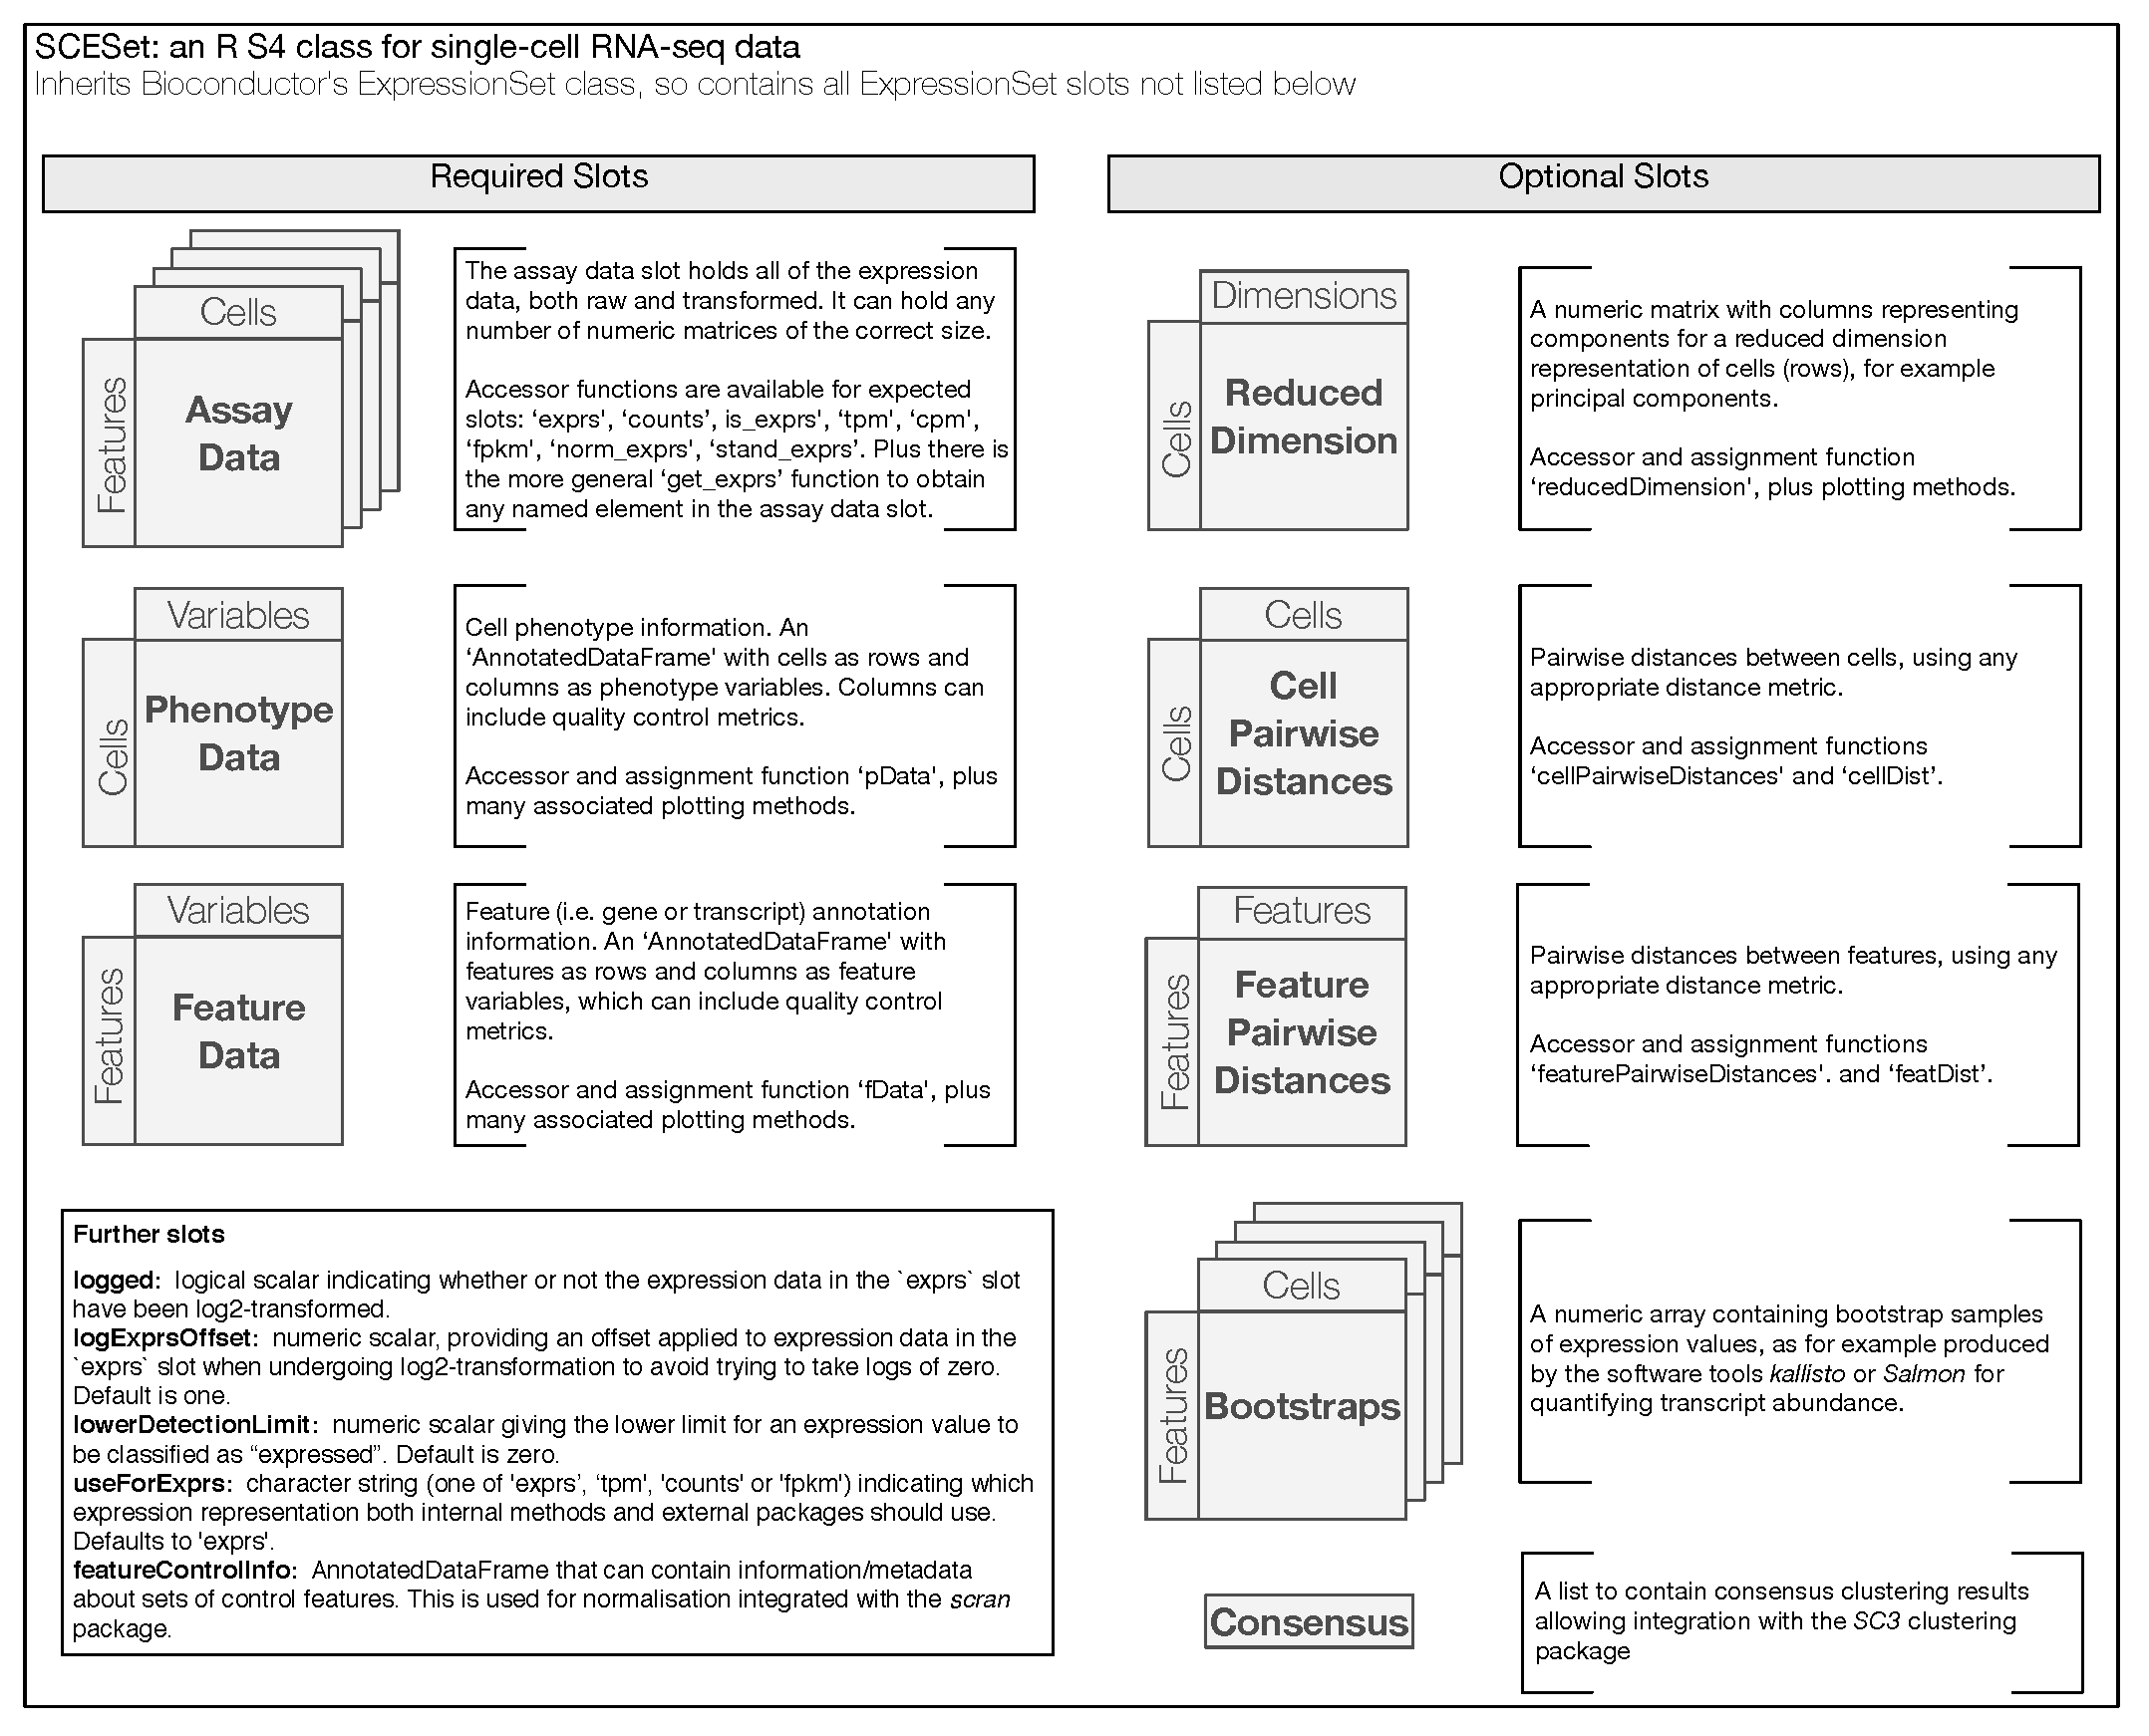
\includegraphics[width=0.95\textwidth]{figures/sceset_outline.pdf}}
\caption{An overview of the SCESet class that underpins the \emph{scater} package. Building on Bioconductor's ExpressionSet class, it is a fully-featured, sophisticated and flexible data class tailored to scRNA-seq data.}\label{fig:02}
\end{figure}


\begin{figure}[!tpb]
\centerline{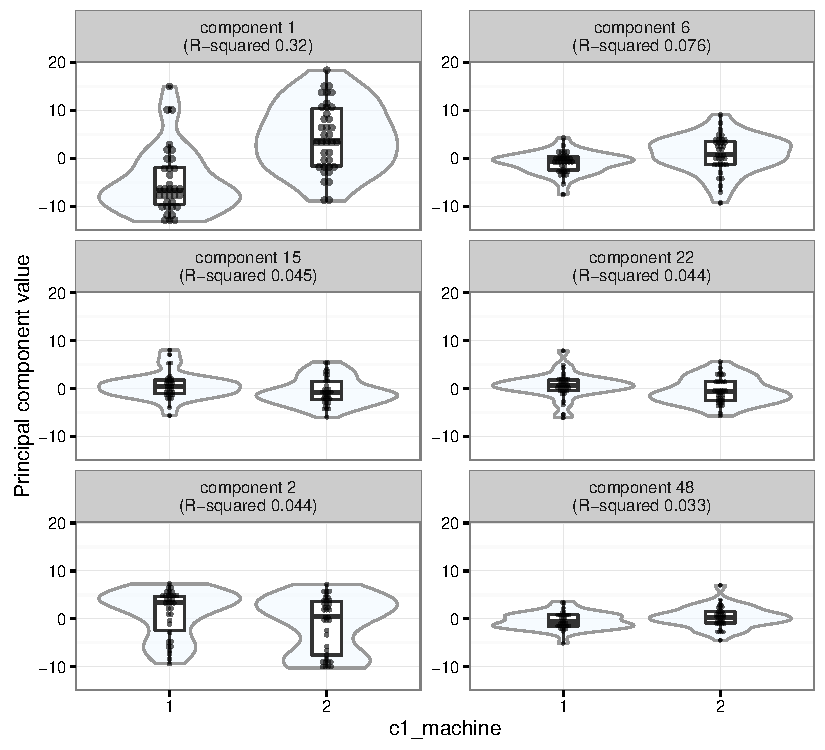
\includegraphics[width=0.7\textwidth]{figures/find-pcs_c1_machine.pdf}}
\caption{A QC plot produced by the plotQC function in \emph{scater} showing violin, scatter- and boxplots of principal component values against the C1 machine used for each cell for the six principal components most strongly correlated with C1 machine used.}\label{fig:plotqc-c1-machine}
\end{figure}


\begin{figure}[!tpb]
\centerline{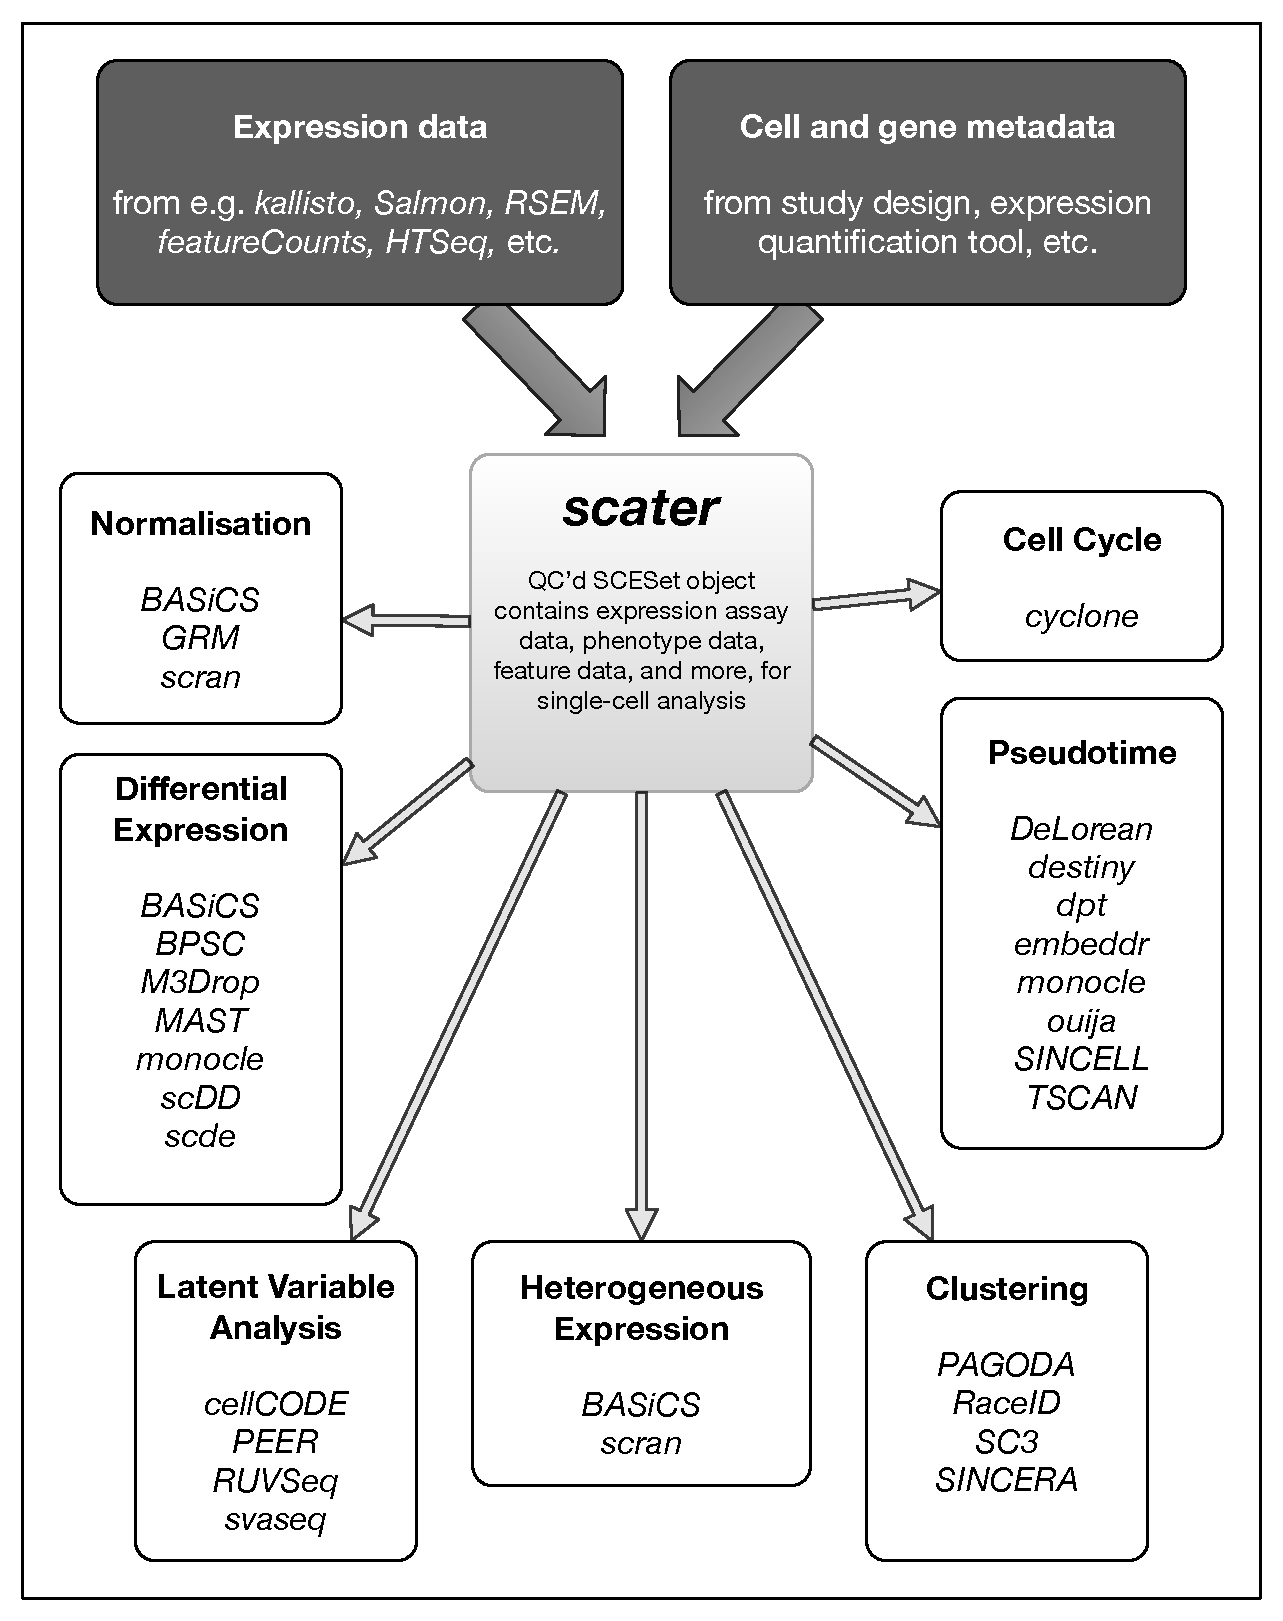
\includegraphics[width=0.95\textwidth]{figures/scater_ecosystem.pdf}}
\caption{An overview of the \emph{scater} ecosystem. The SCESet class in \emph{scater} acts as a convenient hub for datasets so that many other methods and tools implemented in R can be applied.}\label{fig:scater-eco}
\end{figure}


\begin{figure}[!tpb]
\centerline{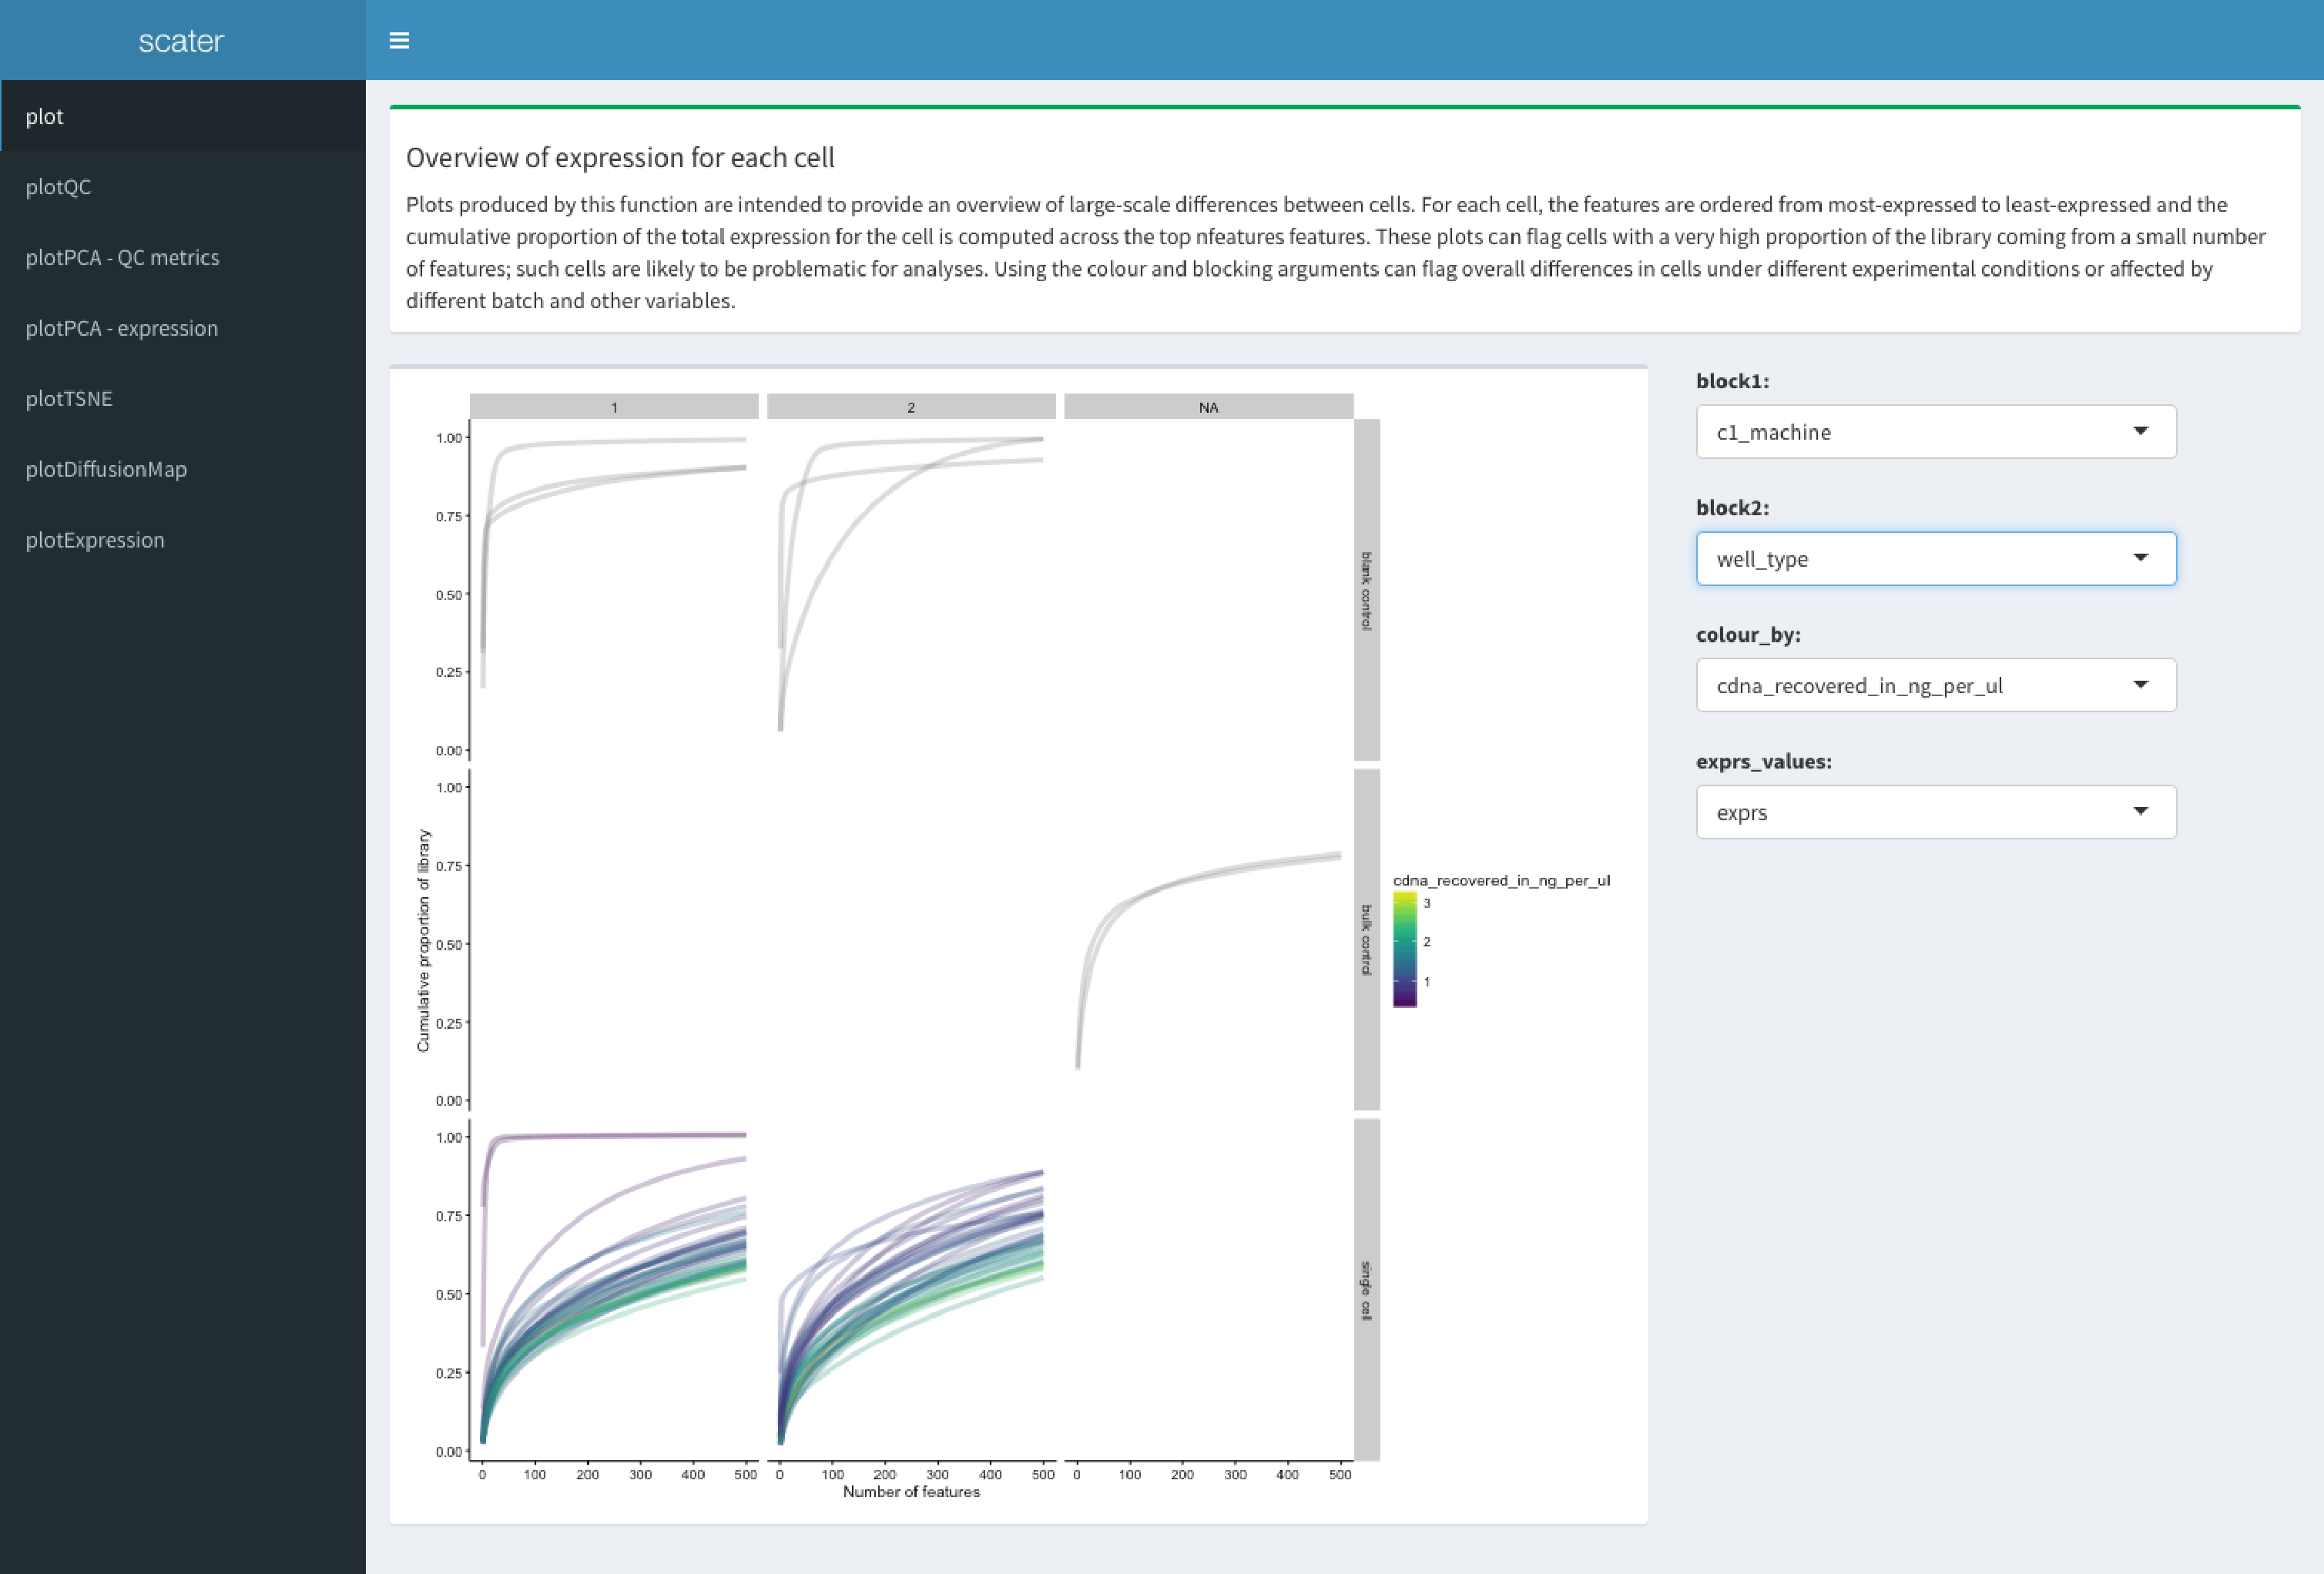
\includegraphics[width=0.95\textwidth]{figures/scater_gui_landing_page.pdf}}
\caption{The landing page for the \emph{scater} graphical user interface (GUI).}\label{fig:scater-gui-landing}
\end{figure}


\begin{figure}[!tpb]
\centerline{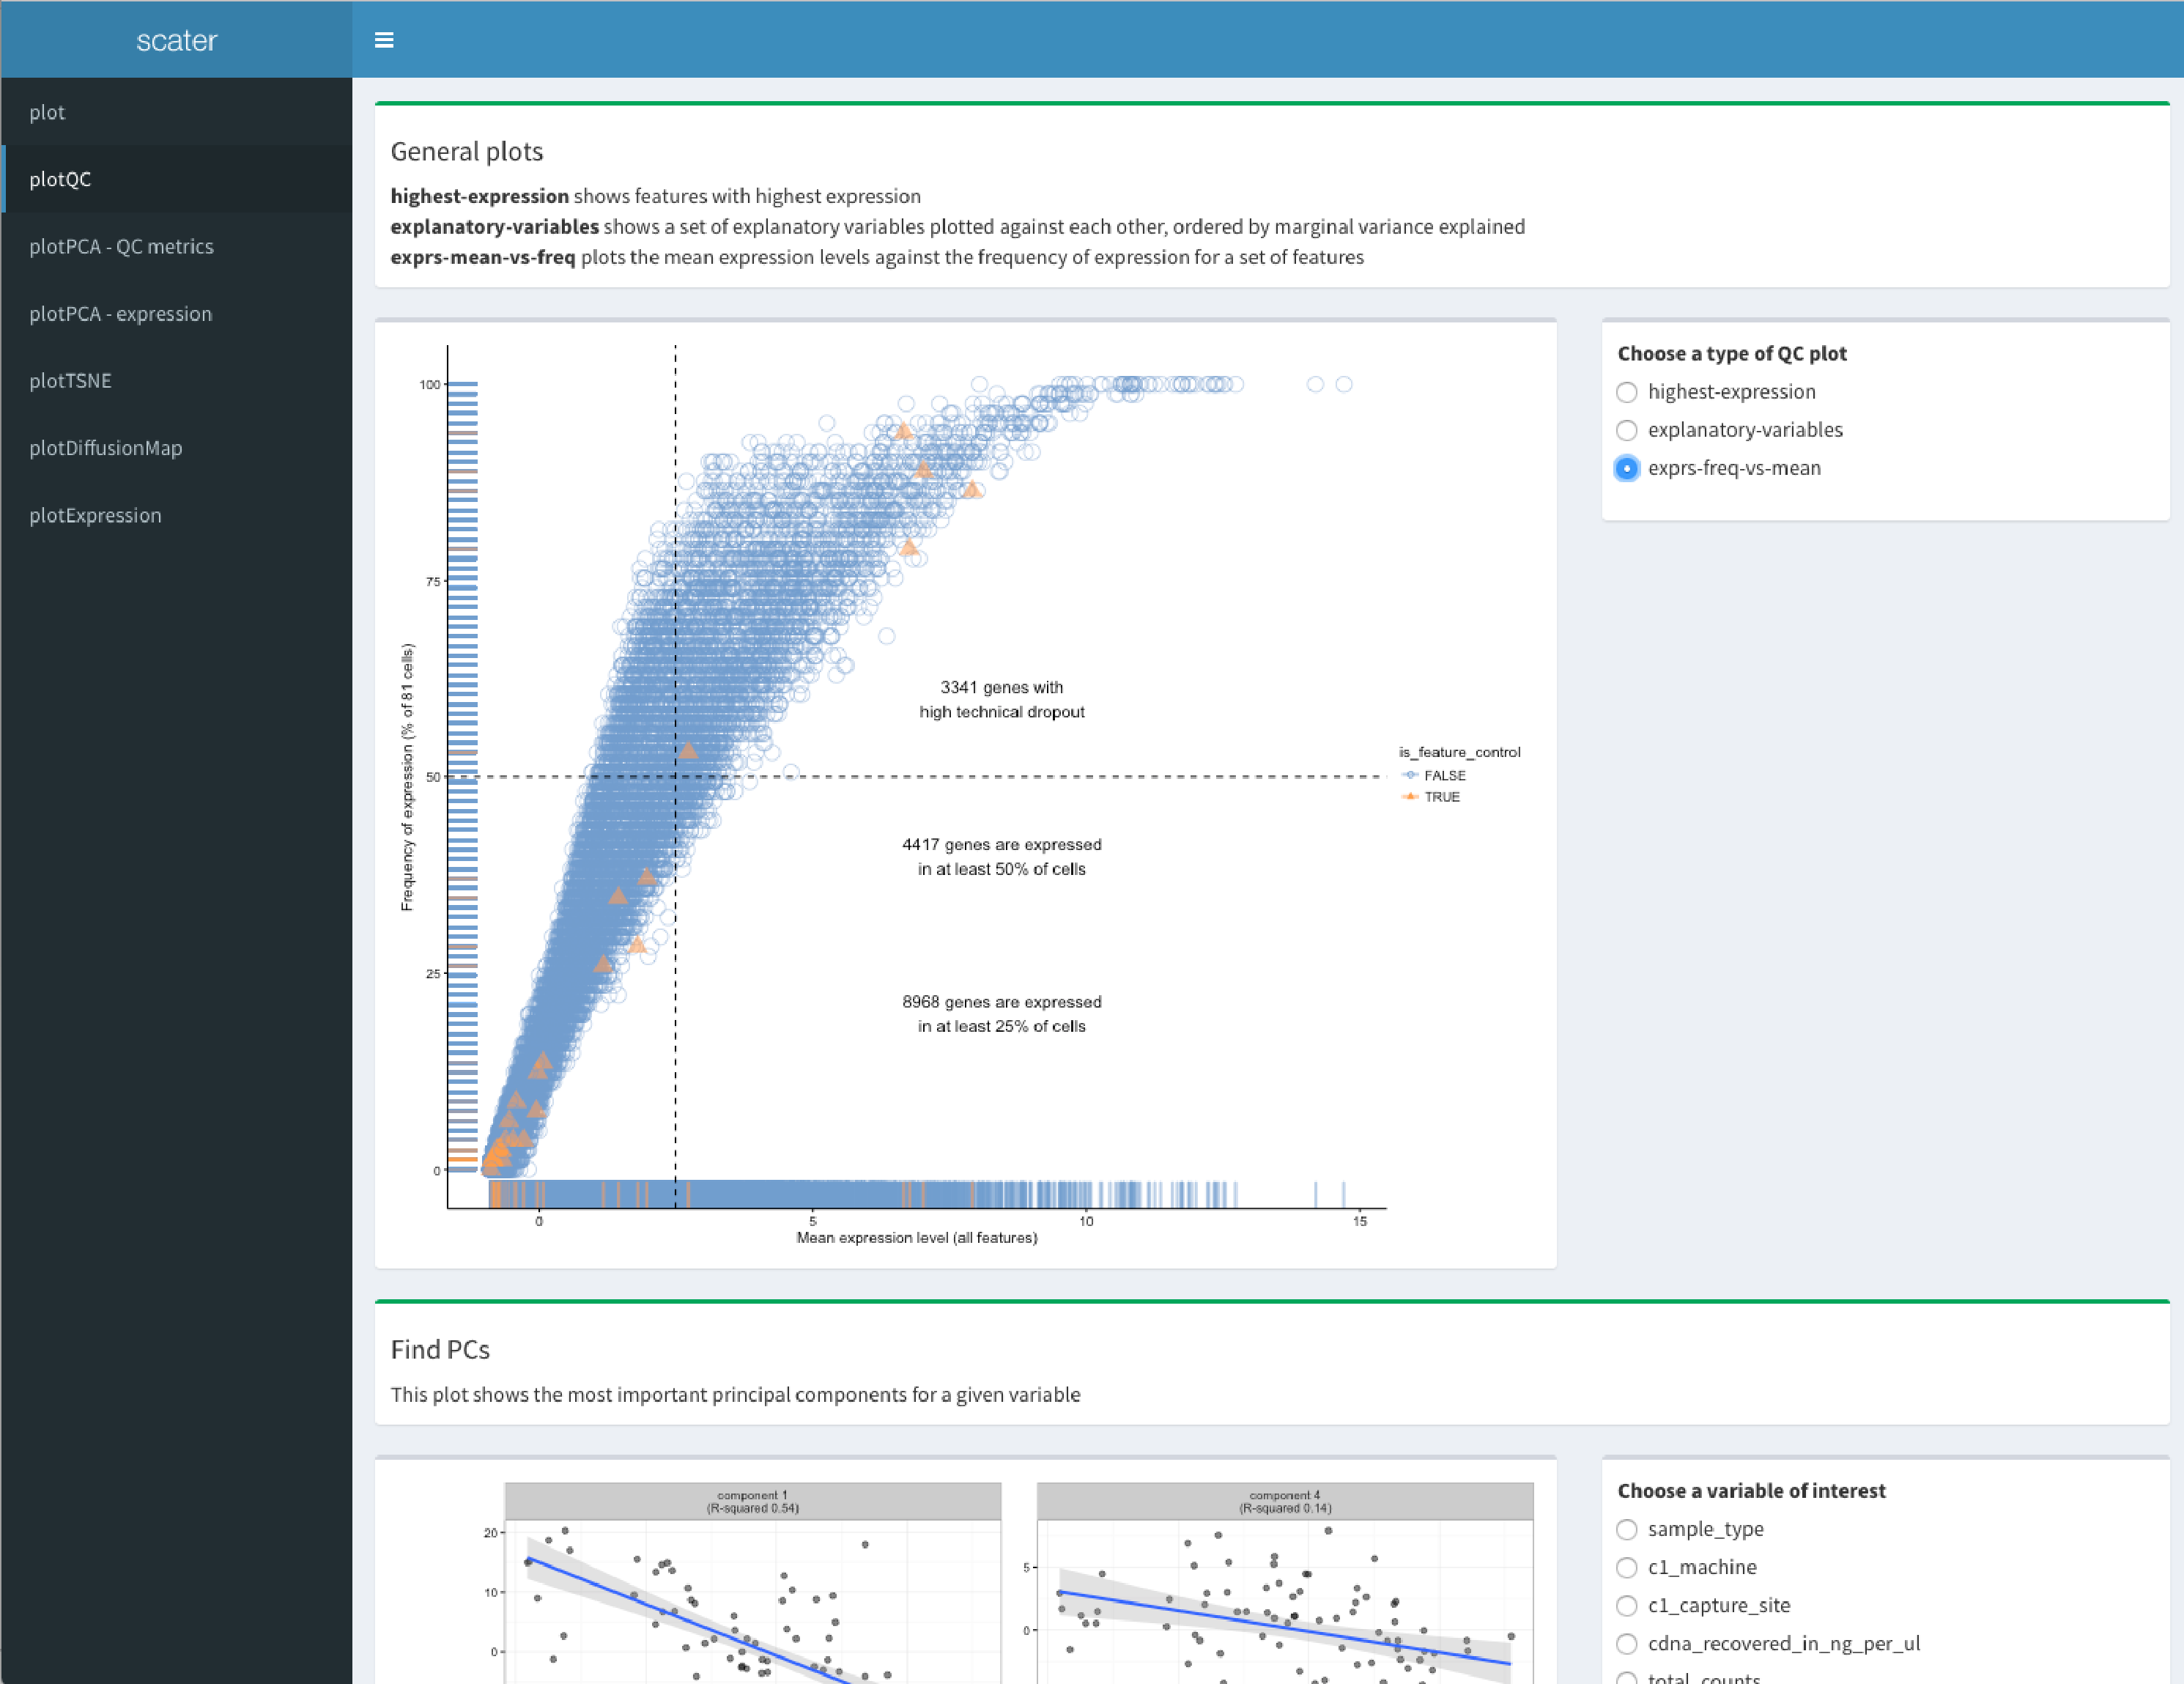
\includegraphics[width=0.95\textwidth]{figures/scater_gui_plotqc.pdf}}
\caption{The \texttt{plotQC} page for the \emph{scater} graphical user interface (GUI).}\label{fig:scater-plotqc}
\end{figure}


\begin{figure}[!tpb]
\centerline{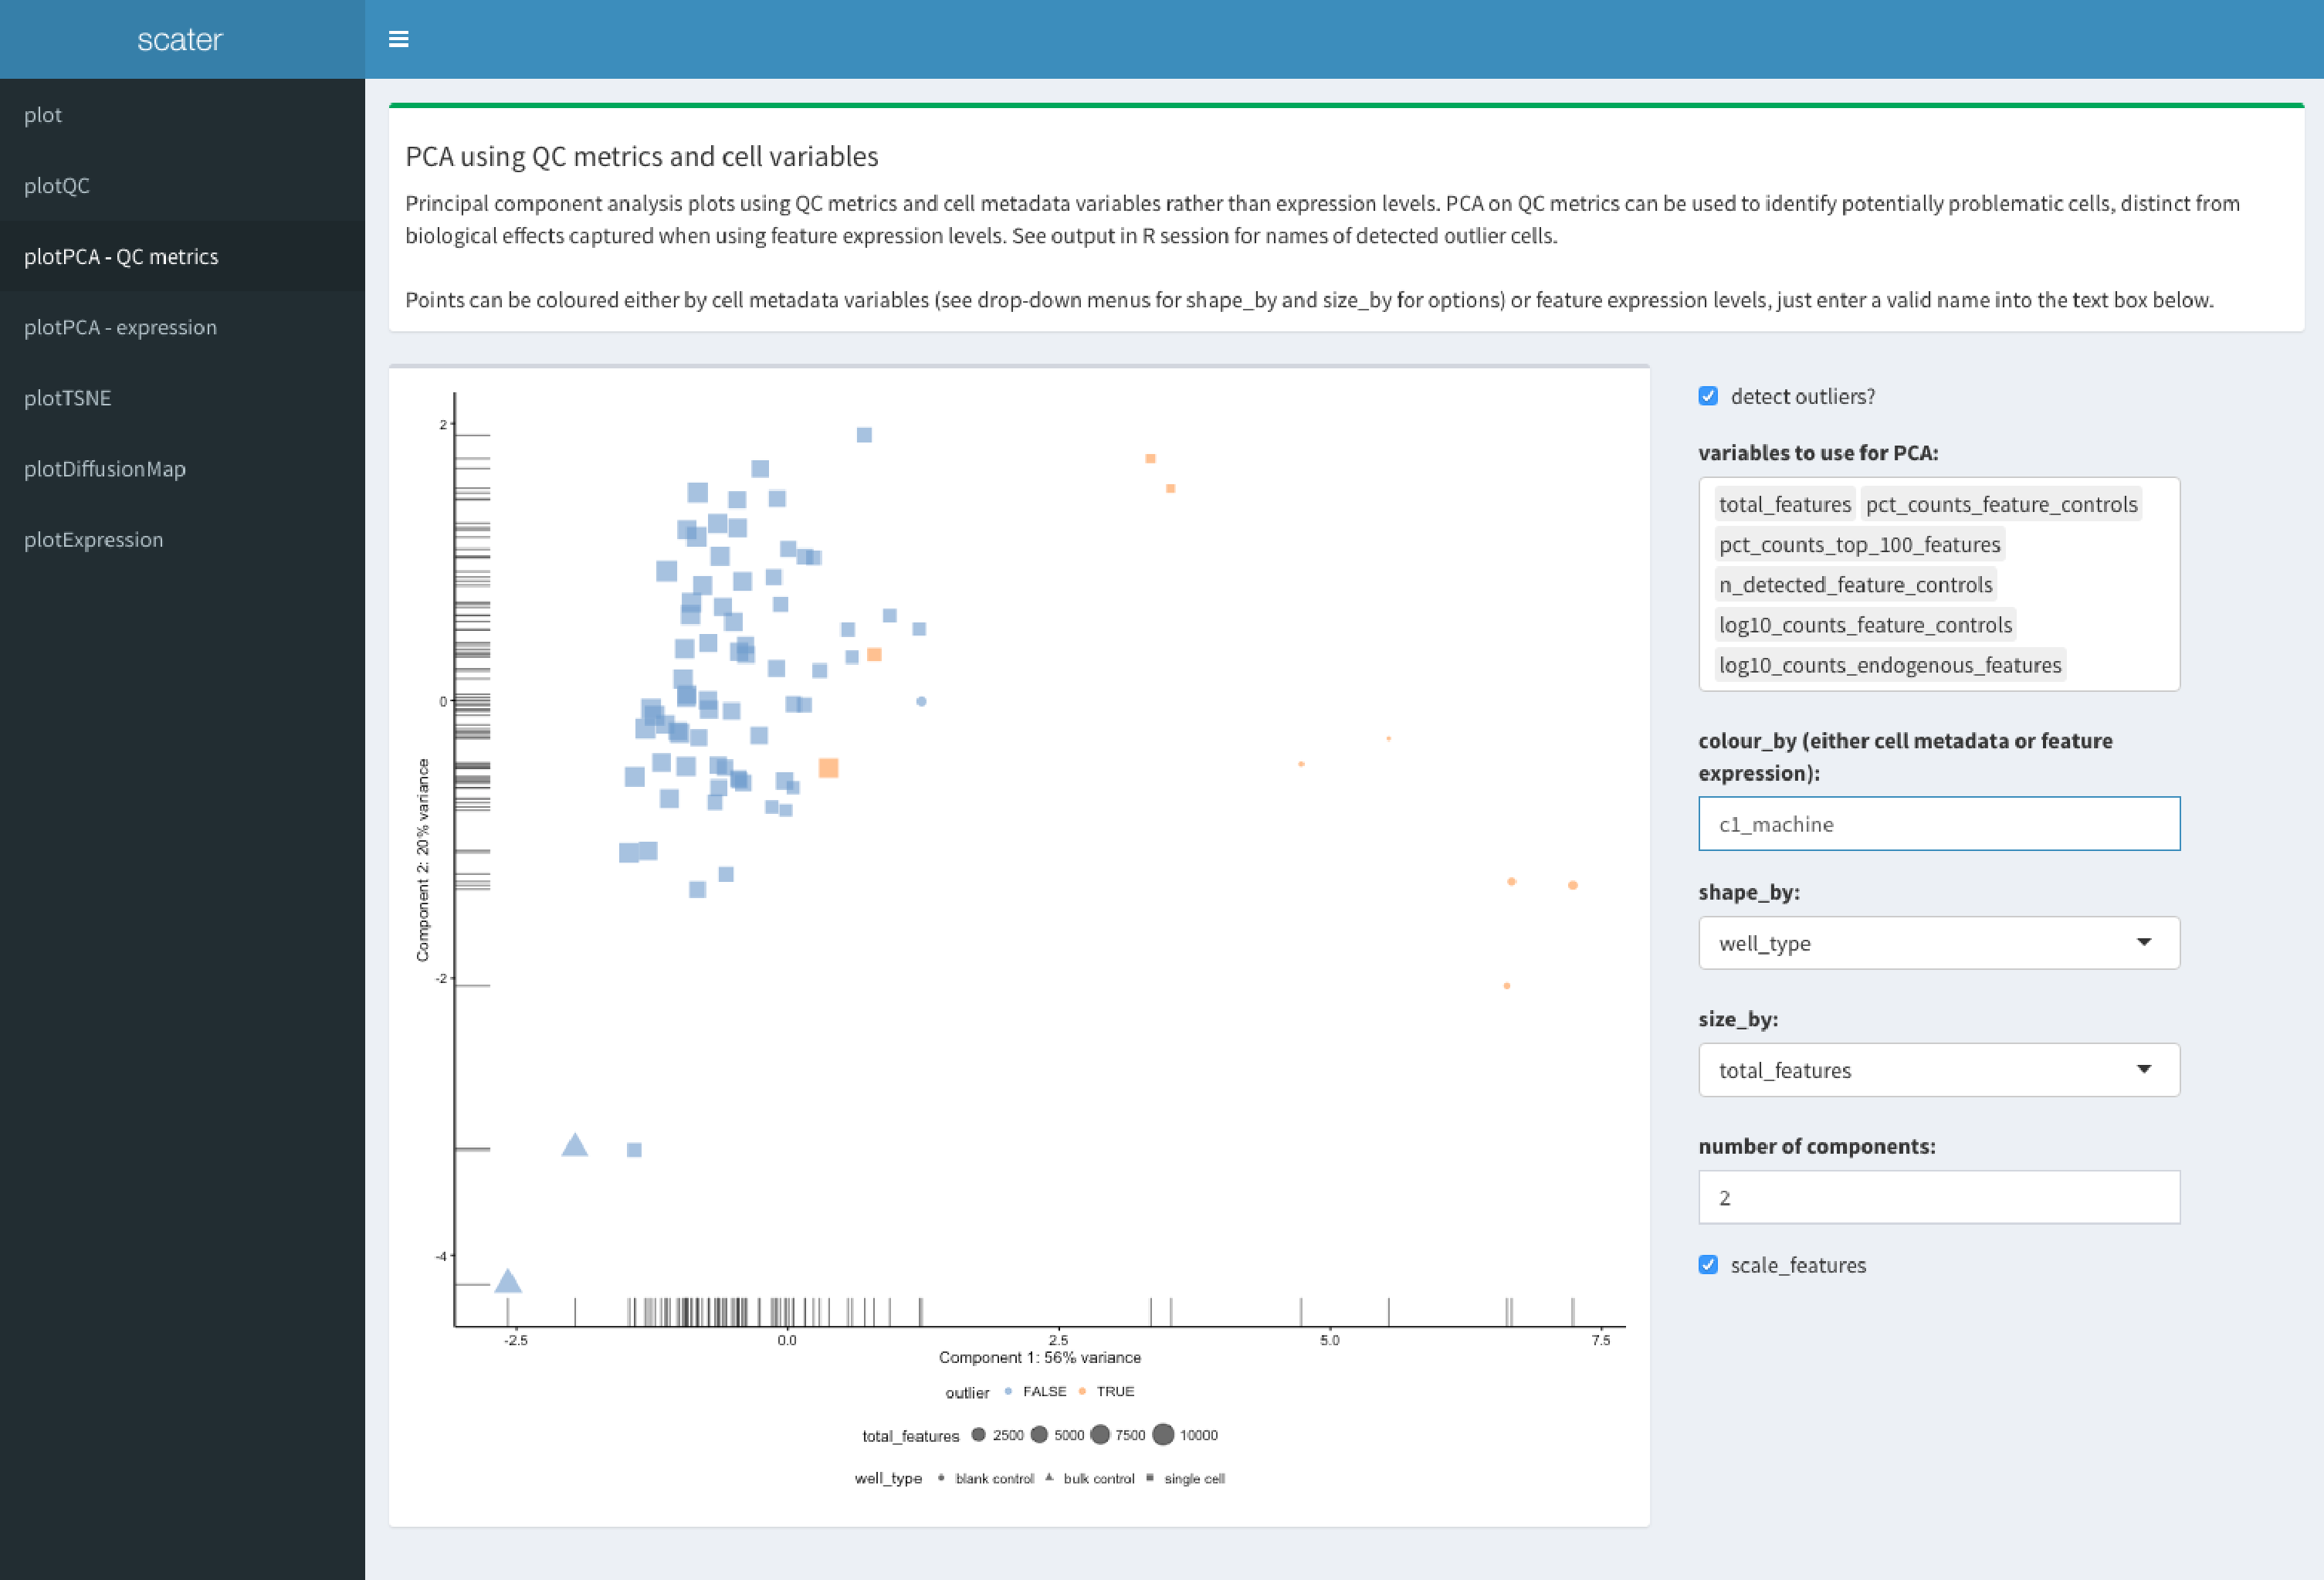
\includegraphics[width=0.95\textwidth]{figures/scater_gui_pca_qc.pdf}}
\caption{The \texttt{plotPCA - QC} page for the \emph{scater} graphical user interface (GUI).}\label{fig:scater-pca-qc}
\end{figure}



\bibliographystyle{natbib}
%\bibliographystyle{achemnat}
%\bibliographystyle{plainnat}
%\bibliographystyle{abbrv}
%\bibliographystyle{plain}
%\bibliographystyle{bioinformatics}
\bibliography{main}


\end{document}
